\documentclass{article}
\usepackage[utf8]{inputenc}
\usepackage{amsmath}
\usepackage{graphicx}
\graphicspath{ {images/} }

\newcommand{\specialcell}[2][c]{%
	\begin{tabular}[#1]{@{}l@{}}#2\end{tabular}}

\begin{document}
\begin{titlepage}
	\begin{center}
		\vspace*{0.5cm}
		
\includegraphics[width=0.4\textwidth]{bme}\\		
		Budapesti Műszaki és Gazdaságtudományi Egyetem\\
		Villamosmérnöki és Informatikai Kar\\
		Automatizálási és Alkalmazott Informatikai Tanszék\\		
		\vspace{3.2cm}
		\huge
		\textbf{Járó robot készítése}
		\vspace{1.5cm}\\
		\large
		Babics Mátyás	
		\vfill		
		Konzulens\\
		Nagy Ákos\\
		\vspace{1.5cm}		
		Budapest, 2018		
	\end{center}
\end{titlepage}
\section{Bevezetés}
A feladat egy négylábon járó robot elkészítése volt. A megvalósításhoz szükség volt megtervezni a robot modelljét. A kialakítás pókokhoz hasonlít, de nyolc helyett négy lábbal. A mozgást biztosító szervók vezérlését egy mikrokontrollerrel ellátott áramkör biztosítja. Ennek feladata az akkumlátor feszültségét megfelelő szintre konvertálnia és összeköttetést teremteni a mikrokontroller és perifériák között. A mozgáshoz bonyolult algoritmusokat matematikailag leírva C++-ban implementálva a mikrokontroller futtatja.
\begin{figure*}[h]
	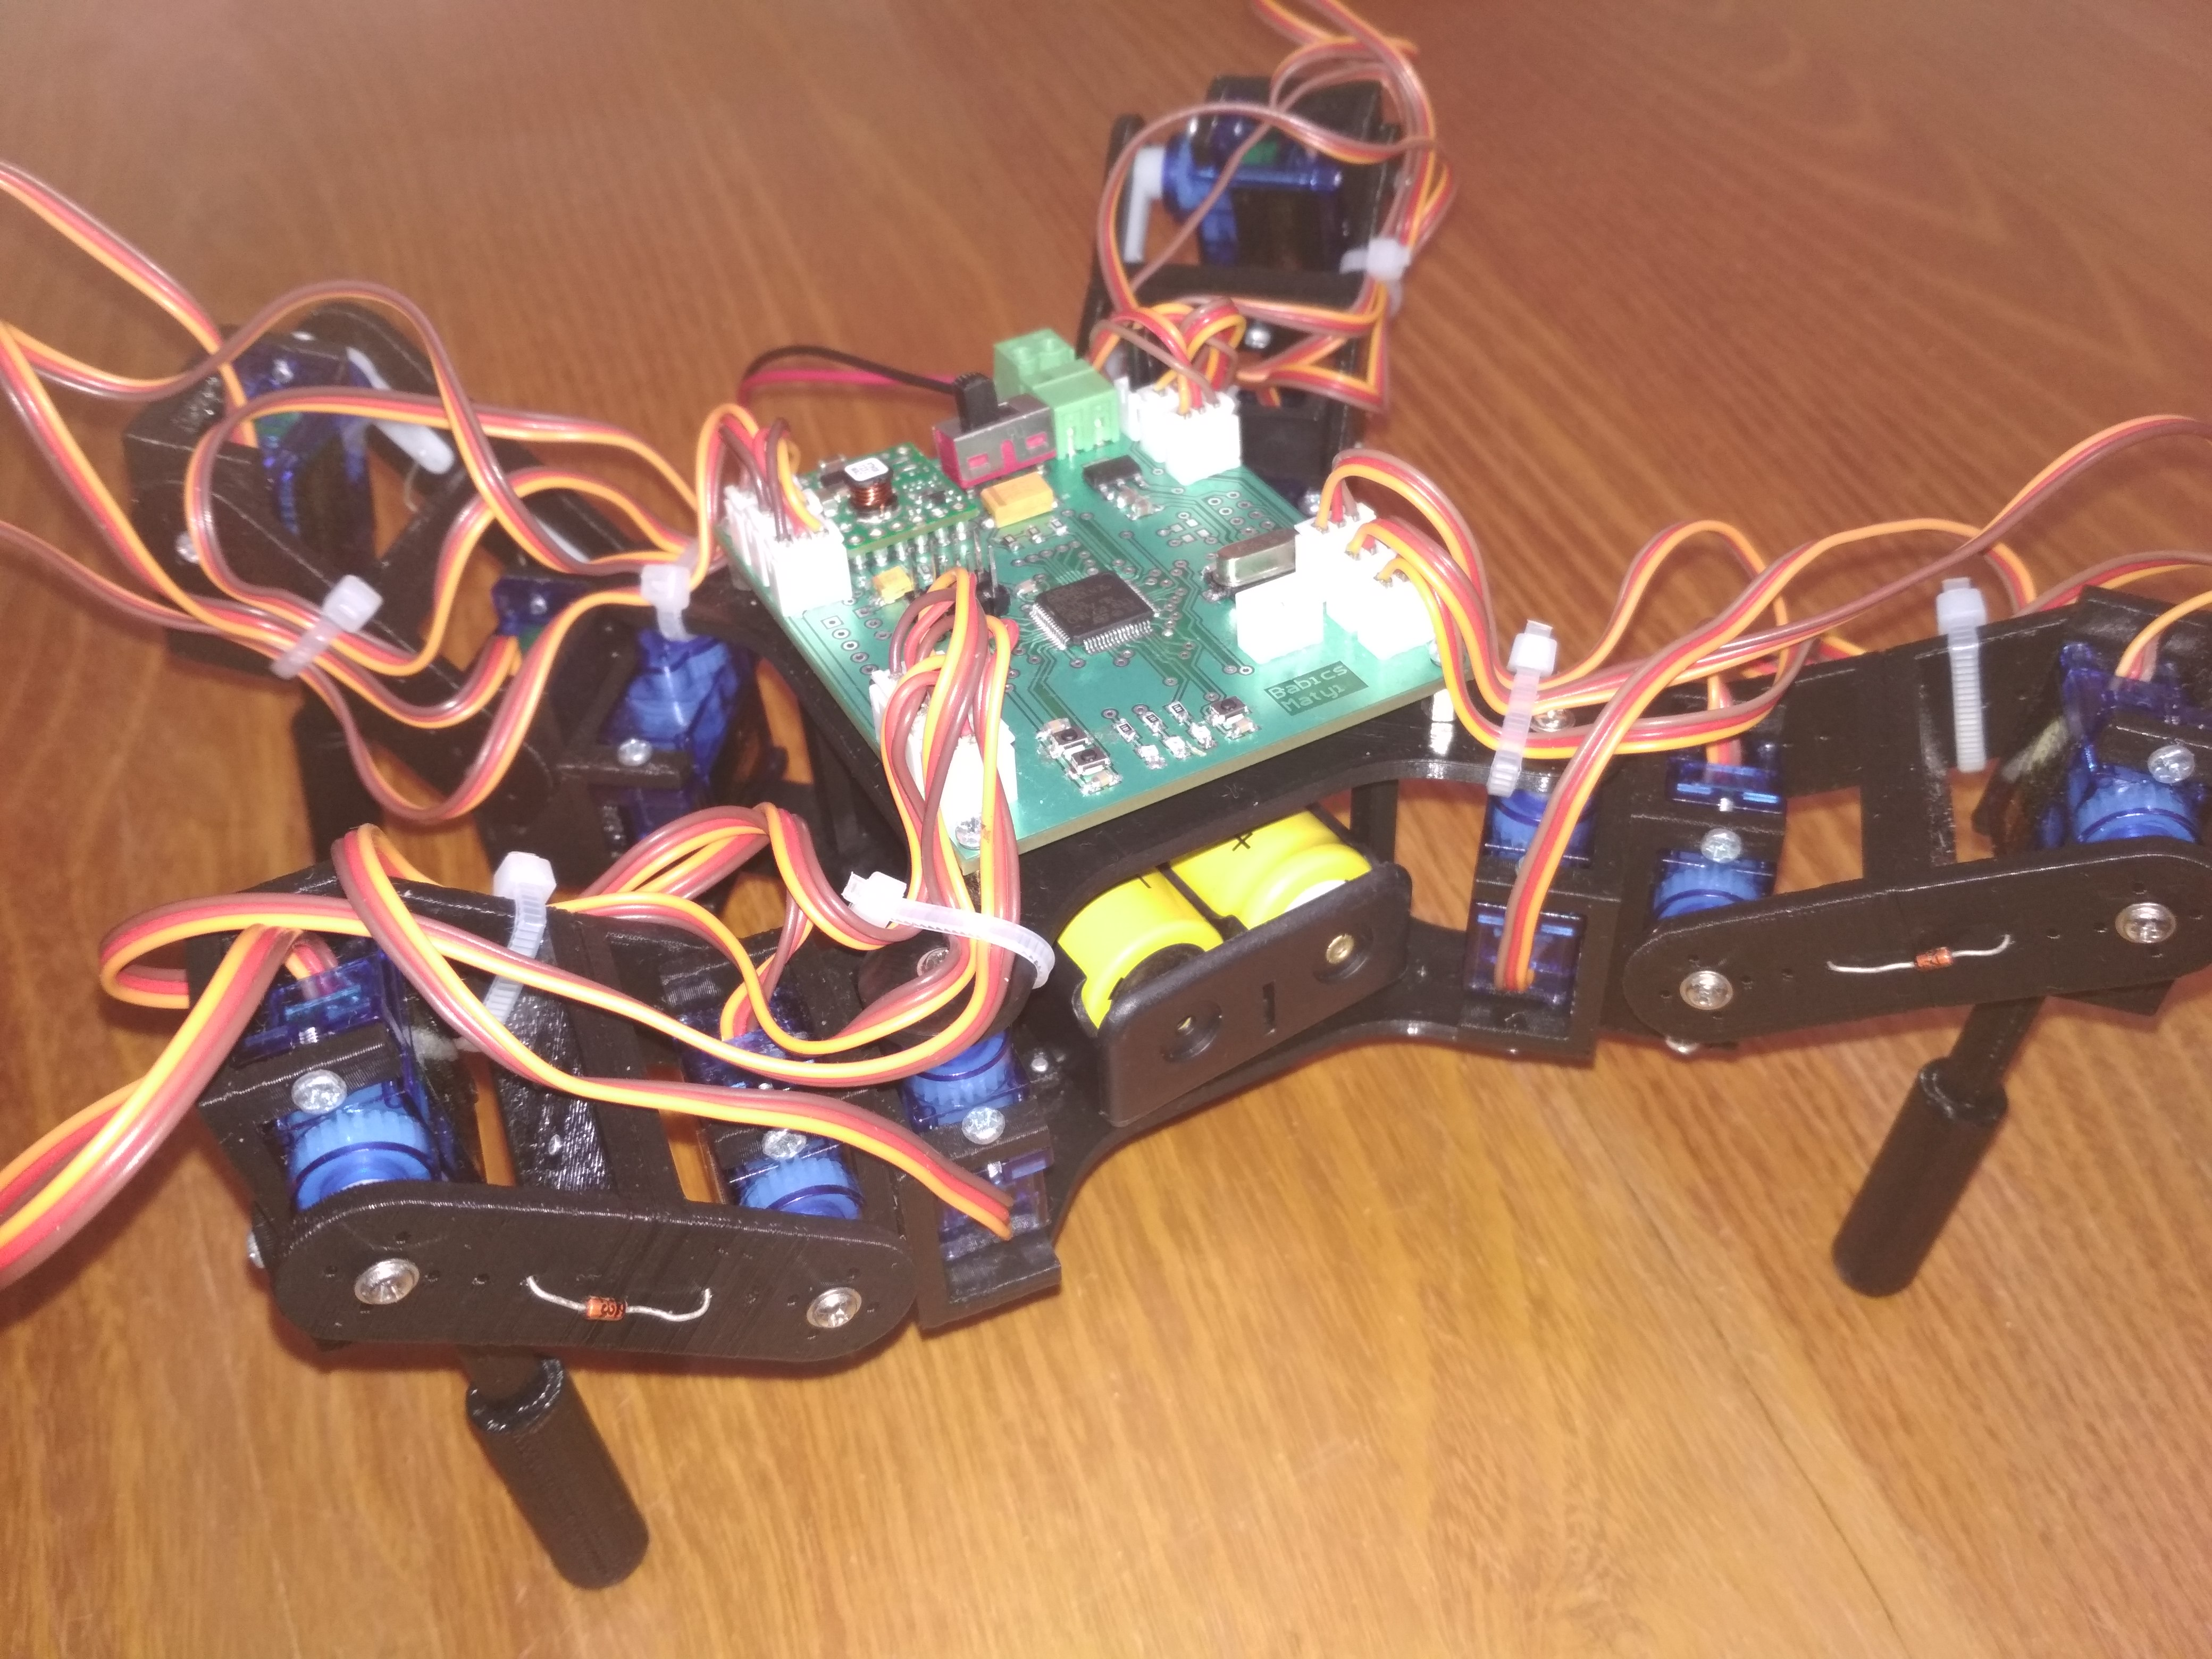
\includegraphics[width=\textwidth]{quad}
\end{figure*}
\newpage

\section{Model}
A robot modellje 3D nyomtatással készült, amihez a tervek Autodesk Inventorral készültek. A modell fő részei a teste és 4 lába, amik további 3 részre bonthatók. Az egyes részek tengelyek mentén el tudnak forogni egymáshoz képest. A lábaknak 3 szabadságfokuk van a tetszőleges pozíció eléréséhez.
\begin{figure}[h]
	\centering
	\begin{minipage}{0.3\textwidth}
		\centering
		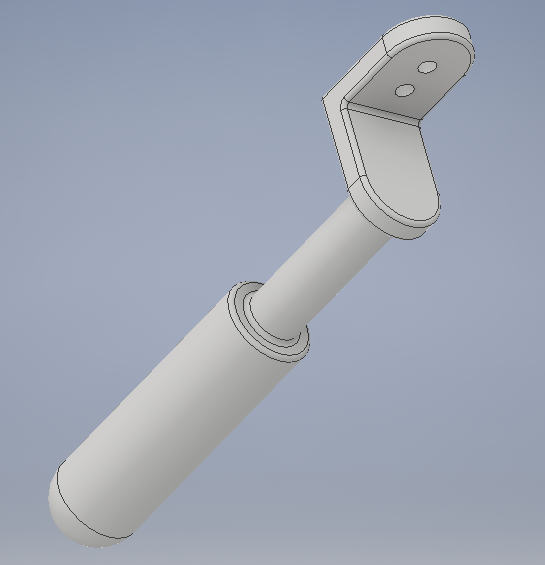
\includegraphics[width=\textwidth]{labveg}
		\caption{Láb vége}
	\end{minipage}\hfill
	\begin{minipage}{0.3\textwidth}
		\centering
		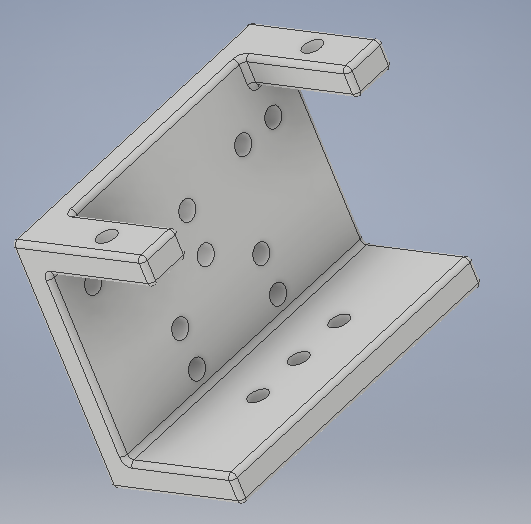
\includegraphics[width=\textwidth]{motortarto}
		\caption{Motortartó}
	\end{minipage}\hfill
	\begin{minipage}{0.3\textwidth}
		\centering
		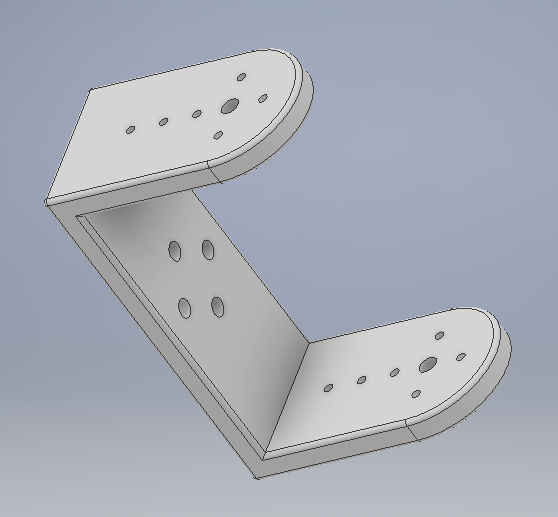
\includegraphics[width=\textwidth]{labszar}
		\caption{Lábszár}
	\end{minipage}
\end{figure}
\begin{figure}[h]
\centering
\begin{minipage}{0.3\textwidth}
	\centering
	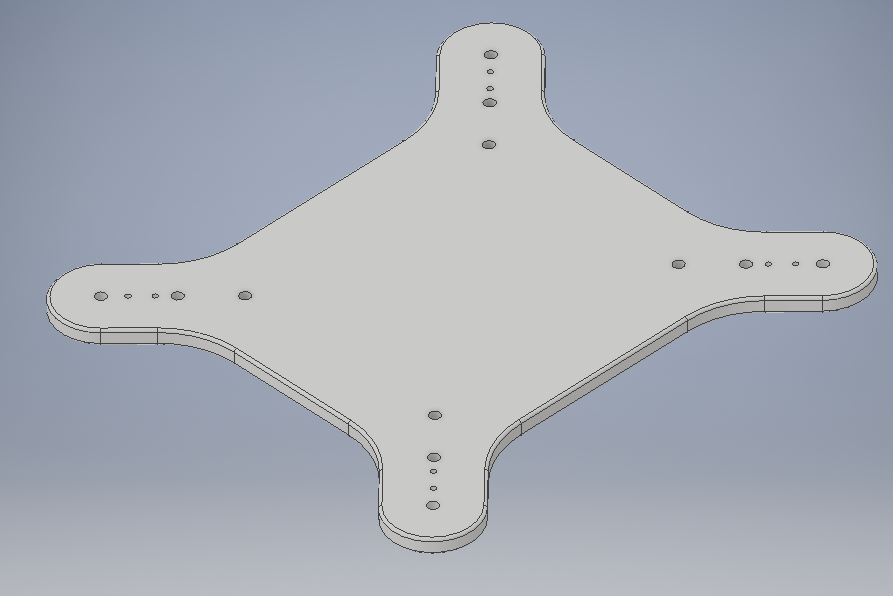
\includegraphics[width=\textwidth]{testfo}
	\caption{Test fő része}
\end{minipage}\hfill
\begin{minipage}{0.3\textwidth}
	\centering
	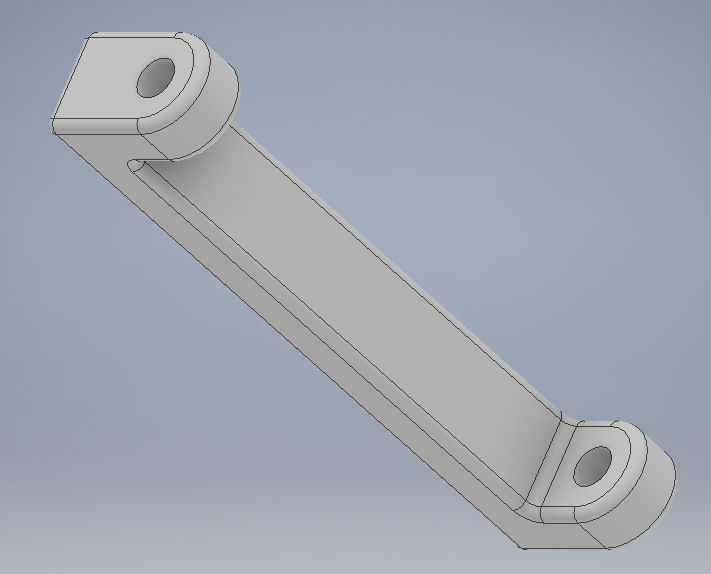
\includegraphics[width=\textwidth]{testtarto}
	\caption{Test fő részek között támasz}
\end{minipage}\hfill
\begin{minipage}{0.3\textwidth}
	\centering
	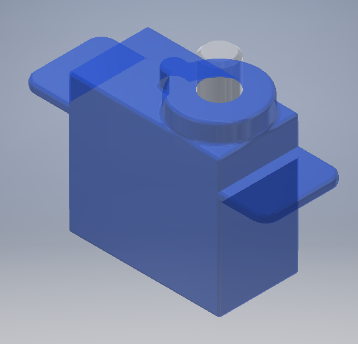
\includegraphics[width=\textwidth]{motor}
	\caption{Motor}
\end{minipage}
\end{figure}
\\
Az alkatrészeken látható nagyobb lyukak 2mm, a kisebbek 1mm átmérőjűek. A részeket 2mm-es csavarok tartják össze a nagyobb lyukakba csavarva. A kisebb lyukak a használt motorok fejéhez lettek mérve. A fejet megfogva a motor forgó részéhez rögzítik magukat mozgást eredményezve. Az elemek vastagsága 3mm.
A láb vége elem egy motortartóhoz illeszkedik, meghosszabbítva a láb végső szakaszát 80mm-re. Vége lekerekített, így orientációja nem sokat befolyásolja a talajjal érintkezés pontos helyzetét a testhez képest. A robottól független tökéletlenségek miatt, mint például egyenetlen talaj, praktikusan nem lehetséges kiszámolni a láb pontos helyzetét. 
A motortartó feladata a motor hozzácsatolása a modell többi részéhez. A motor fülein 2mm-es lyukak vannak, amikkel rögzíthető az álló rész. A tartó ezeken fogja a motort.
Lábszárból 2-t egymáshoz csavarva H alakot kapva adódik a láb középső része. A tengelyek között 30mm távolságot tart. A két fül között 34mm van, ide illeszkedik a motortartó és a motor.
A test fő részéből 2 van egymás fölött, közöttük 4 támasz helyezkedik el. A test 96mm hosszú és 86mm széles. A támaszok 34mm hosszúak, ugyanakkora helyet adva a motortartó-motor együttesnek, mint a lábszár. A lábak a testen látható négy elálló fülön helyezkednek el.
\begin{figure}[h]
	\centering
	\begin{minipage}{0.45\textwidth}
		\centering
		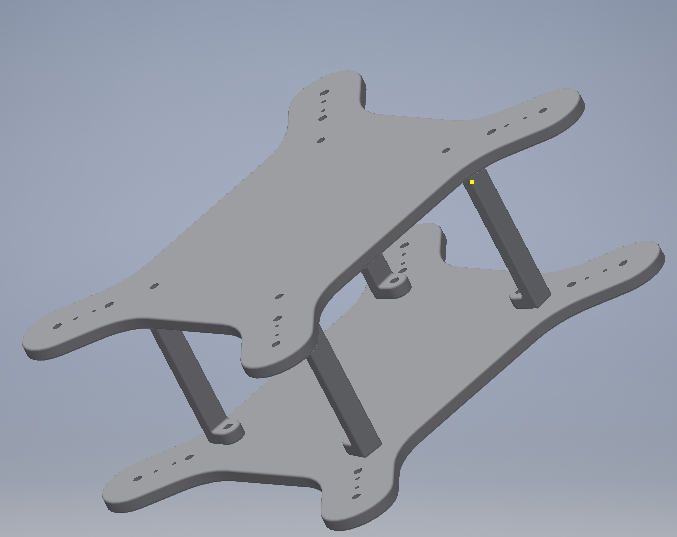
\includegraphics[width=\textwidth]{fulltest}
		\caption{Test}
	\end{minipage}\hfill
	\begin{minipage}{0.45\textwidth}
		\centering
		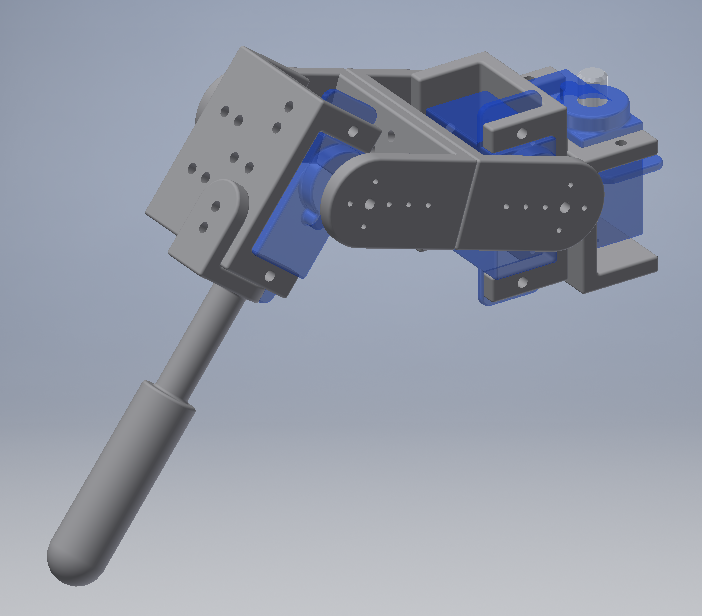
\includegraphics[width=\textwidth]{fulllab}
		\caption{Láb}
	\end{minipage}
\end{figure}
\begin{figure}[h]
\centering
\begin{minipage}{0.45\textwidth}
	\centering
	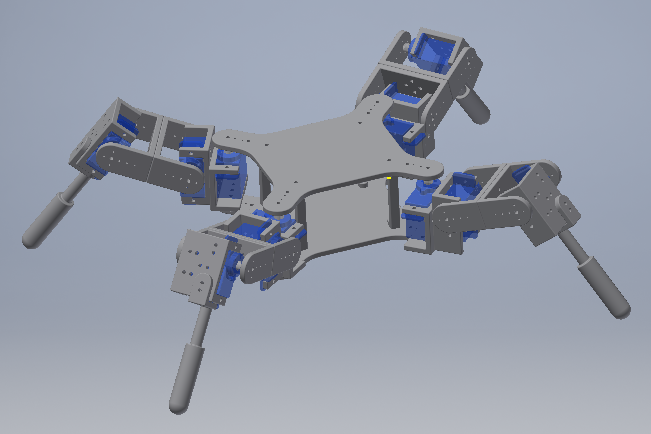
\includegraphics[width=\textwidth]{fullquad}
	\caption{Robot modellje}
\end{minipage}\hfill
\begin{minipage}{0.45\textwidth}
	\centering
	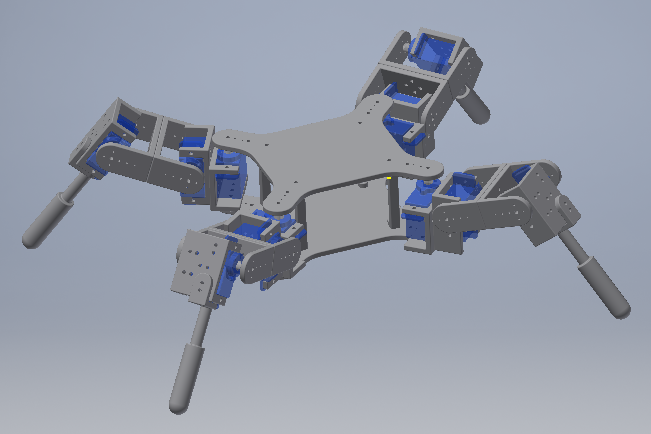
\includegraphics[width=\textwidth]{fullquad}
	\caption{Robot készen}
\end{minipage}
\end{figure}
A modell dizájnjához egy létező quadruped adta az inspirációt. A méretek meghatározásának fő szempontja a motorok és vezérlést biztosító nyák mérete volt. A végtagok a testhez képest hosszúak lettek, hogy messze elérjenek. A láb középső része (30mm) lényegesen rövidebb a végső részénél (80mm), így a robot teste a talaj fölött maradhat úgy is, hogy a térde a test fölött van. Ez tisztán kinézet kérdése, valójában nagyobb térfogat lenne lefedhető egyforma tengelytávolságokkal, viszont járásnál semmi megkötést nem jelent.
\section{Hardware}
A hardware egy nyomtatott áramkörre készült el. A vezérlést egy STM32L476RET6 típusú mikrokontroller végzi. Ehhez órajelet egy 8MHz-es kristály oszcillátor biztosítja. A mikrokontrolleren 12 timer kimenet PWM módban vezéreli az SG-90 típusú motorokat. A tápellátást két sorosan kapcsolt 3.7V-os Li-ion akkumulátor adja. A feszültség meglétét egy kék LED jelzi. A feszültség egy harmadoló osztón csatlakozik a mikrokontroller egy analóg bemenetére. A 7.4V-ból egy PTH08T231WAD típusú konverter 5V-ot állít elő a motoroknak. 5V-ból egy TS1117BCW-3.3 típusú LDO 3.3V-ot állít elő a mikrokontrollernek.
Ezeken kívül van a nyákon:
\begin{itemize}
\item 3 sárga LED tetszőleges jelzéshez, és 1 piros akkumulátor töltöttsége jelzéséhez
\item 3 nyomógomb, 1 resethez, 2 a mikrokontrollerre bemenetnek
\item 5V, 3.3V, GND kivezetés
\item UART kommunikáció külső eszközzel
\item Programozó interfész
\item ESP alapú wifi modul
\item Sharp sensor távolságérzékelő
\item 8 GPIO
\end{itemize}
\subsection{Mikrokontroller}
A választás egy STM32L476RET6 típusú mikrokontrollerre esett. A választás szempontjai:
\begin{itemize}
\item Megfelelő számú kimenet, ebből 12 PWM
\item Elegendő számítási teljesítmény, FPU 
\item Tokozás
\item Fejlesztői környezet
\item Ismeretség
\item Ár
\end{itemize}
A választott mikrokontroller mindnek eleget tesz. A 12 PWM kimenetet TIM1, TIM2 és TIM3 időzítők biztosítják, mindegyik 4-4 kimeneten. USART3-n kommunikál a wifi modullal, UART4-en a kívülről illesztett egységgel, mint például számítógéppel. Az akkumulátor töltöttségét és a távolságérzékelő analóg kimenetét az ADC1 1-es és 2-es csatornáin figyeli. A PB0-PB7 lábak ki vannak vezetve tetszőleges felhasználásra. Az egyéb illesztett ki- és bemenetek elhelyezés szerint kedvező GPIO lábakra csatlakoznak.
\subsection{Motor}
A motorok SG-90 típusú mikroszervók. Táplálásuk 5V-ról történik. Vezérlésükhöz 50Hz-es PWM jelet kell bemenetükre adni adatlap szerint 1-2ms-es kitöltési tényezővel, ami hatására $0-180^{\circ}$-ban fordulnak. A lábak pozícióba állításához ez kifejezetten előnyös. A motor továbbá kis méretű, könnyű és szolgáltat elegendő nyomatékot.
\subsection{Táp}
Az energiaellátást két sorba kapcsolt 18350 Li-ion akkumulátor szolgálja, kapcsolóval megszakítható. Ennek feszültsége 7.4-8.2V.
Ebből egy PTH08T231WAD DCDC konverter 5V-ot állít elő. A konverter bemeneti feszültsége 4.5V-tól 14V-ig terjedhet, kimeneti feszültsége egy ellenállással állítható. 160R-os ellenállás használatával a pontos kimenet 5.02V. Mivel a 7.4V-ot ez az átalakító, egy ellenállással sorosan kapcsolt LED és 3-mal leosztva a mikrokontroller egy analóg, 5V toleráns lába kapja meg, a tápellátás értéke felmehet 14V-ig, viszont 9.9V fölött az analóg bemeneten információ veszik el. Nagyobb feszültség hatására egyéb mellékhatás a tápellátást jelző LED erősebb fénye. A konverter maximális kimeneti árama 6A, hatásfoka 1A-től 85\% fölött van, és akár 95\%-ot is elérhet.
A mikrokontrollerhez szükséges 3.3V-ot egy TS1117BCW-3.3 típusú LDO állítja elő 5V-ból. Ugyan itt rosszabb a hatásfok, a konverter kis mérete és a rajta átfolyó kis teljesítmény miatt esett rá a választás.
\subsection{Nyák}
A motorok csatlakozója 3-mas csoportokban a nyák négy sarkánál vannak. A táp a nyák hátulján (képen jobb oldal) érkezik, és itt konvertálja át 5V-ra és 3.3V-ra. Itt helyezkedik el a kapcsoló, a bekapcsolást jelző kék LED és az akkumulátor merülését jelző piros LED. A 3 nyomógomb és 3 sárga LED a nyák elején (képen bal oldal) vannak. A mikrokontroller a nyák közepére került, hogy a legegyszerűbben ki lehessen vezetni a lábakat az adott eszközökhöz. E fölött és alatt van a kristály oszcillátor és a kivezetések programozáshoz és illeszthető eszközökhöz.
\begin{figure}[h]
\centering
	\begin{minipage}{0.3\textwidth}
		\centering
		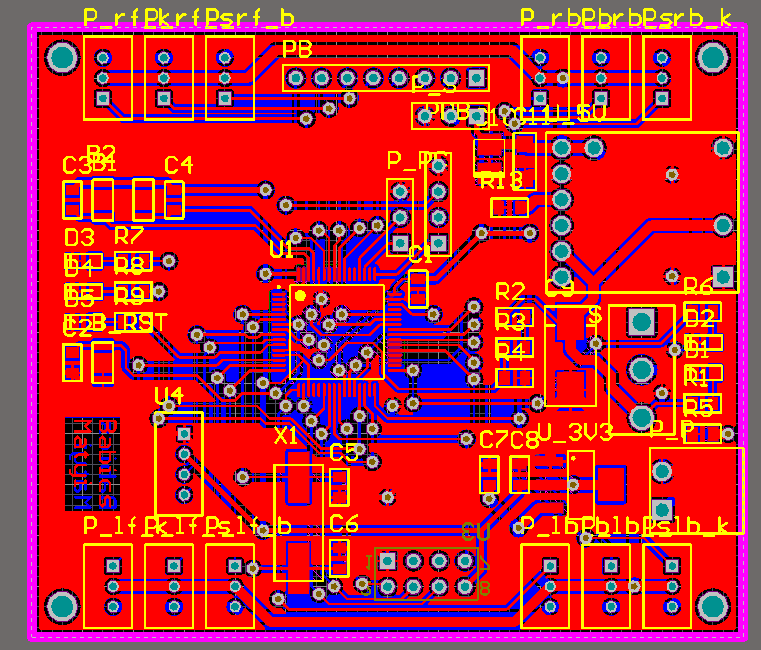
\includegraphics[width=\textwidth]{nyakfelso}
		\caption{Nyák felső rétege}
	\end{minipage}\hfill
	\begin{minipage}{0.3\textwidth}
		\centering
		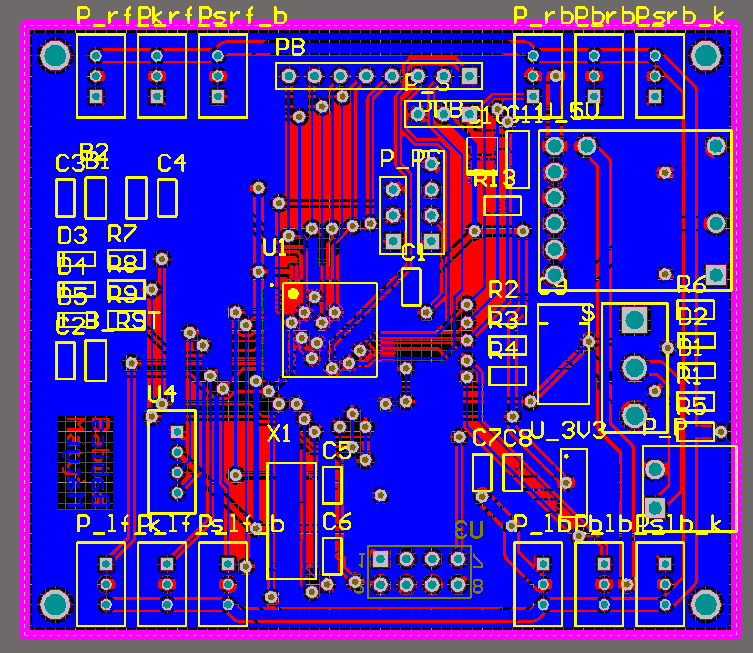
\includegraphics[width=\textwidth]{nyakalso}
		\caption{Nyák alsó rétege}
	\end{minipage}\hfill
	\begin{minipage}{0.3\textwidth}
		\centering
		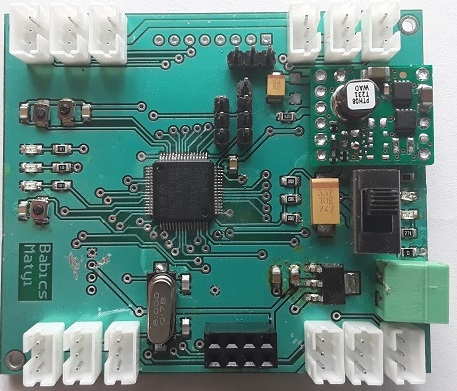
\includegraphics[width=\textwidth]{nyakforr}
		\caption{Forrasztott nyák}
	\end{minipage}
\end{figure}
\section{Algoritmusok}
\subsection{Direkt geometria}
\subsubsection{Transzformációs mátrixok}
A quadruped középpontját origónak tekintve, ahol X irány jobbra, Y fölfele és Z előre mutat, a robot egy lábának csuklóinak és merev részeinek transzformációs mátrixai:

$$
\begin{pmatrix}
	1&0&0&d_x\\
	0&1&0&d_y\\
	0&0&1&d_z\\
	0&0&0&1
\end{pmatrix}	
\begin{pmatrix}
	C_1&0&S_1&0\\
	0&1&0&0\\
	-S_1&0&C_1&0\\
	0&0&0&1
\end{pmatrix}	
\begin{pmatrix}
	1&0&0&0\\
	0&1&0&0\\
	0&0&1&d_1\\
	0&0&0&1
\end{pmatrix}	
\begin{pmatrix}
	1&0&0&0\\
	0&C_2&-S_2&0\\
	0&S_2&C_2&0\\
	0&0&0&1
\end{pmatrix}
$$
$$
\begin{pmatrix}
	1&0&0&0\\
	0&1&0&0\\
	0&0&1&d_2\\
	0&0&0&1
\end{pmatrix}	
\begin{pmatrix}
	1&0&0&0\\
	0&C_3&-S_3&0\\
	0&S_3&C_3&0\\
	0&0&0&1
\end{pmatrix}	
\begin{pmatrix}
	1&0&0&d_{3x}\\
	0&1&0&0\\
	0&0&1&d_3\\
	0&0&0&1
\end{pmatrix}
$$
\subsubsection{Paraméterek}
Paraméterek értéke radiánban ill. mm-ben:\\\\
\begin{tabular}{ | l | c | c | c | c | c | c | c | c | c | c | }
	\hline
	láb&$\alpha_1$&$\alpha_2$&$\alpha_3$&$d_x$&$d_y$&$d_z$&$d_1$&$d_2$&$d_3$&$d_3x$\\
	\hline
	jobb első&$\pi/4$&$0$&$\pi/4$&$35$&$21$&$40$&$18$&$40$&$80$&$4$\\
	\hline
	jobb hátsó&$3\pi/4$&$0$&$\pi/4$&$35$&$21$&$-40$&$18$&$40$&$80$&$-4$\\
	\hline
	bal első&$-\pi/4$&$0$&$\pi/4$&$-35$&$21$&$40$&$18$&$40$&$80$&$-4$\\
	\hline
	bal hátsó&$-3\pi/4$&$0$&$\pi/4$&$-35$&$21$&$-40$&$18$&$40$&$80$&$4$\\
	\hline
\end{tabular}\\\\
Az $\alpha_n$ értékek az elfordulás offsetét jelzik. Ezek jelentősége, hogy a megvalósításnál alkalmazott motorok $-\pi$ és $\pi$ között tudnak mozogni, és ilyen offsetek mellett tud a robot lába legkényelmesebben pozíciókba állni.\\
A $d_x$, $d_y$ és $d_z$ az első motor tengelyébe való eltolás a második motor tengelyének magasságában,	$d_1$ az első és második, $d_2$ a második és utolsó motor tengelye közti eltolás, $d_3$ az utolsó motor tengelye és a láb vége közti eltolás, $d_{3x}$ pedig a láb vége és első motor tengelye közti oldalirányú eltolás, aminek iránya egybeesik a második és harmadik tengelyek irányával, így az első motor után mindegy hol vesszük figyelembe. A paraméterek jobban láthatóak a \ref{fig:param} képen.
\begin{figure}[h]
\begin{minipage}{0.9\textwidth}
	\caption{Lábak paraméterei}
	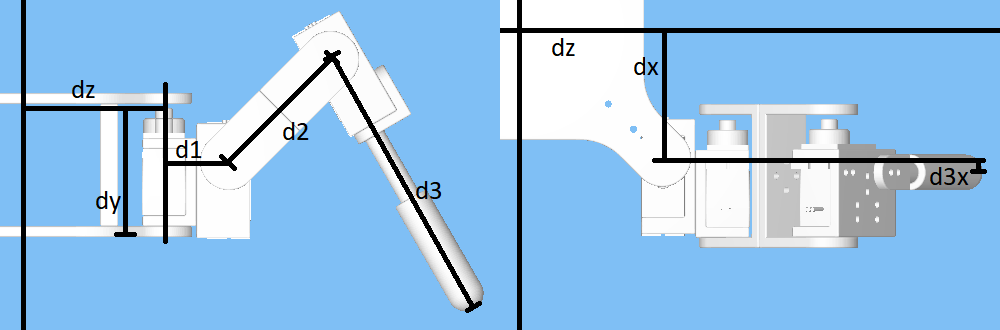
\includegraphics[width=\textwidth]{quad_params}
	\label{fig:param}
\end{minipage}
\end{figure}

\subsubsection{Számolás}
A transformációs mátrixokat összeszorozva egy láb rotaciós mátrixa és pozícióvektora:
$$
\begin{pmatrix}
C_1&S_1S_{23}&S_1C_{23}\\
0&C_{23}&-S_{23}\\
-S_1&C_1S_{23}&C_1C_{23}
\end{pmatrix}
=
Rot
$$
$$
\begin{pmatrix}
C_1d_3x+S_1C_{23}d_3+S_1C_2d_2+S_1d_1+d_x\\
-S_{23}d_3-S_2d_2+d_y\\
-S_1d_{3x}+C_1C_{23}D_3+C_1C_2d_2+C_1d_1+d_z
\end{pmatrix}
=
\begin{pmatrix}
p_x\\
p_y\\
p_z
\end{pmatrix}
$$
\\
A rotációs mátrix nem szükséges, a cél, hogy a láb vége az általunk mondott pozícióba kerüljön. Habár arra oda kell figyelni, hogy a lábfej ne alulról érintse a talajt, ami fizikailag lehetetlen. A megvalósításból adódóan ez csak akkor lenne lehetséges, ha az egész robot a talaj alatt lenne.
	
\subsection{Inverz geometria}
$A sin(\vartheta)+B cos(\vartheta)=D$ egyenlet megoldásai:
\begin{align} \label{eq:trigeq}
\vartheta = arctan \left( \frac{A D\pm B\sqrt{A^2+B^2-D^2}}{B D\mp A\sqrt{A^2+B^2-D^2}} \right)
\end{align}
Az $arctan$ függvény helyett használható az $atan2()$ függvény, ami külön kapja meg a számlálót és nevezőt, és $2\pi$ periodicitással adja meg a szöget.
\subsubsection{Első szög}
Direkt geometriából ismertek a következő egyenletek:
\begin{align*}
C_1 d_{3x}+S_1 (C_{23} d_3+C_2 d_2+d_1)+d_x=p_x
\end{align*}
\begin{align*}
-S_1 d_{3x}+C_1 (C_{23} d_3+C_2 d_2+d_1)+d_x=p_z
\end{align*}
Ezekből:
\begin{align*}
\frac{C_1}{S_1}d_{3x}+(C_{23} d_3+C_2 d_2+d_1)=\frac{p_x-d_x}{S_1}
\end{align*}
\begin{align*}
\frac{-S_1}{C_1}d_{3x}+(C_{23} d_3+C_2 d_2+d_1)=\frac{p_z-d_z}{C_1}
\end{align*}
A két egyenletet kivonva egymásból és megszorozva $C_1 S_1$-gyel:
\begin{align*}
(S_1^2+C_1^2 ) d_3x=C_1 (p_x-d_x )-S_1 (p_z-d_z)
\end{align*}
Itt a \eqref{eq:trigeq} egyenletbe behelyettesítve $A=d_z-p_z$, $B=p_x-d_x$ és $D=d_3x$ értékeket kapható az első csukló állása.
\begin{align}
\vartheta_1 = arctan \left( \frac{(d_z-p_z) d_3\pm (p_x-d_x)\sqrt{(d_z-p_z)^2+(p_x-d_x)^2-d_3^2}}{(p_x-d_x) d_3\mp (d_z-p_z)\sqrt{(d_z-p_z)^2+(p_x-d_x)^2-d_3^2}} \right)
\end{align}
Mivel $D\cong0 (4 mm)$, $\vartheta_1\cong arctan\left(\frac{\pm B}{\mp A}\right)$, így a két megoldás közel $\pi$-ben tér el egymástól. Emiatt, és mert a határok közelében a többi láb mozgásterét zavarná, és így azt nem éri, elég a $-\pi/2$, $\pi/2$ közötti eredménnyel folytatni a számolást.
\subsubsection{Második szög}
\begin{align*}
C_{23} d_3+C_2 d_2=\frac{p_x-d_x-C_1 d_{3x}}{S_1} -d_1=l
\end{align*}
\begin{align*}
S_{23} d_3+S_2 d_2=d_y-p_y
\end{align*}
$C_{23}$-at és $S_{23}$-at kifejezve:
\begin{align}\label{eq:c23eq}
C_{23}=\frac{l-C_2 d_2}{d_3}
\end{align}
\begin{align}\label{eq:s23eq}
S_{23}=\frac{d_y-p_y-S_2 d_2}{d_3} 
\end{align}
Ezeket négyzetre emelve:
\begin{align*}
C_{23}^2=\frac{l^2+C_2^2 d_2^2-2lC_2 d_2}{d_3^2}
\end{align*}
\begin{align*}
S_{23}^2=\frac{\left(d_y-p_y\right)^2+S_2^2d_2^2-2\left(d_y-p_y\right)S_2d_2}{d_3^2}
\end{align*}
Összeadva a két egyenletet
\begin{align*}
1=\frac{l^2+(C_2^2+S_2^2)d_2^2+\left(d_y-p_y\right)^2-2lC_2 d_2-2\left(d_y-p_y\right)S_2 d_2)}{d_3^2}
\end{align*}
\begin{align*}
e=\frac{l^2+d_2^2+\left(d_y-p_y\right)^2-d_3^2}{2d_2}=lC_2+\left(d_y-p_y\right)S_2
\end{align*}
$A=d_y-p_y$ $B=l$ $D=e$ helyettesítésekkel a képletbe behelyettesítéssel két eredmény kapható.
\begin{align}
\vartheta_2 = arctan \left( \frac{(d_y-p_y) e\pm l\sqrt{(d_y-p_y)^2+l^2-e^2}}{l e\mp (d_y-p_y)\sqrt{(d_y-p_y)^2+l^2-e^2}} \right)
\end{align}
Ezek közül az egyiknél a robot térde felfelé hajlik, a másik megoldásban lefelé. Mindkét megoldással tovább lehet haladni.
\subsubsection{Harmadik szög}
\eqref{eq:c23eq} és \eqref{eq:s23eq} képleteket elosztva egymással, kifejezve $\vartheta_3$-ra
\begin{align}
\vartheta_3=arctan\left(\frac{d_y-p_y-S_2 d_2}{l-C_2 d_2}\right)
\end{align}
\subsubsection{Eredmények értékelése}
Ezáltal kaptunk két megoldást a kívánt pozícióra. Az offseteket kivonva ellenőrizhető, hogy a motor tartományán belül van-e az eredmény. Ha nincs, érvénytelen. Ha a láb hatótávolságán kívül adtunk meg pozíciót, a másodfokú egyenlet diszkriminánsa negatív lesz, nem hozva eredményt.
\subsection{Mozgás}
\subsubsection{Előre haladás}
\begin{figure}[h]
	\begin{minipage}{0.9\textwidth}
		\caption{Kúszó mozgás lépései}
		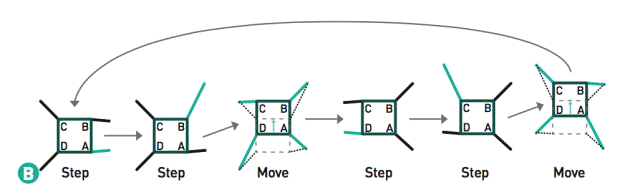
\includegraphics[width=\textwidth]{kuszomozgas}
		\label{fig:mozgas}
	\end{minipage}
\end{figure}
A robot az előre haladást kúszó mozgással valósítja meg. Eközben a robotnak 3 lába mindig a földön van, súlypontja ezek által alkotott háromszögön belülre esik. Ennek a mozgásnak előnye, hogy stabil, bármikor megállhat mozgás közben anélkül hogy eldőlne. Hátránya, hogy lassú. A mozgás hat lépésből áll.\\
A kezdeti állapotot a \ref{fig:mozgas} ábra mutatja. Először jobb hátsó lábát előre viszi 2 egységgel, majd jobb első lábát szintén előre viszi 2 egységgel. Ebből az állapotból előre viszi a testét, vagy a robot inerciarendszere szerint hátra tolja mind a négy lábát 1 egységgel. Ugyanezt megcsinálja a bal lábakkal, majd kezdi elölről. Az egység hossza szabadon választható, határai, hogy az első ábrán látható helyzetben a két jobboldali láb ne ütközzön, és hogy a második ábrán a jobb első láb el tudja érni a helyzetet.
\subsubsection{Forgás}
\begin{figure}[h]
	\begin{minipage}{0.9\textwidth}
		\caption{Forgó mozgás lépései}
		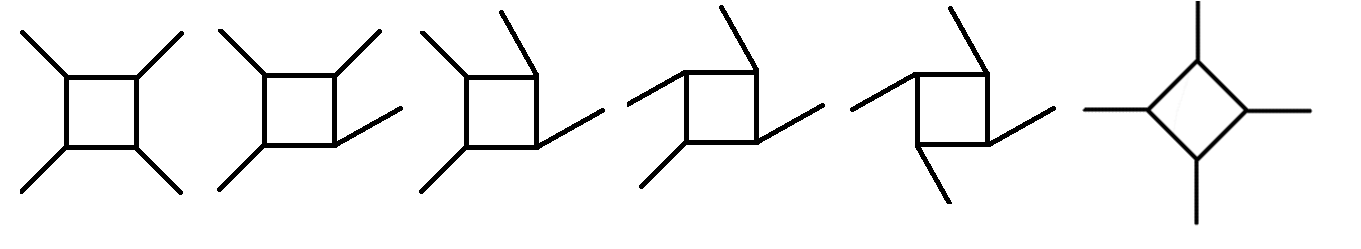
\includegraphics[width=\textwidth]{forgas}
		\label{fig:forgas}
	\end{minipage}
\end{figure}
Forgó mozgás közben a robotnak 3 lába szintén mindig a földön van és a súlypontja a földön lévő lábai által alkotott háromszögön van. Azonban megvalósítás során a súlypont a háromszög egyik oldalára is eshet, vagy azon kívülre, ha nincs pontosan kiegyensúlyozva, így rádől az éppen mozgó lábára. A robot így is tud forogni, viszont dülöngél közben.\\
Mozgás során egyik hátsó lábával kezdve és másik hátsó lábbal befejezve egyesével odább teszi a lábait, majd elfordul a szükséges szögben. A lábai így egy szabályos négyszöget alkotnak. A folyamat a \ref{fig:forgas} ábrán látható. Ez a sorozat 5 lépésből áll és $45^\circ$-ot forgat.
\subsubsection{Lépés}
A robot mozgásának két fajtája van. Vagy egy lábbal lép, vagy az egész teste mozog.\\
Ha egy lábbal lép, akkor a lábát a $-y+(1-(2t-1)^2)*h$ képlet szerinti magasságba helyezi, ahol $y$ a robot hasa távolsága a földtől, $h$ az, amilyen magasra emeli a lábát és $t$ az idő a $[0,1]$ intervallumon, ami jelzi, hol tart a lépésben. Egyenes mozgás közben a síkon a lábak egy egyenes mentén mozognak, forgás közben a robot középpontja körüli kör mentén. Ha ekkor is egyenes mentén mozognának, a láb tövéhez közel vinné el a lábát, ami nem érhető el.\\
Az egész test mozgása a robot szempontjából a lábak együttes mozgatását jelenti. Ilyenkor meghatározza, hogy hova kerül a teste és ezt a mozgást végzi el a lábakon ellentétes előjellel.
\section{Software}
A robot programja C-ben és C++-ban íródott a System Workbench for STM32 Eclipse alapú IDE-ben. Hardware absztrakcióhoz LL könyvtárat használ, ami a HAL könyvtárhoz hasonlóan függvényeket és makrókat ad a hardware kezeléséhez. A perifériák osztályok példányosításával érhetőek el. Burkolót adnak az alsó szintű függvények fölé hogy objektumorientált szemlélet szerint lehessen programozni.
\subsection{Perifériák}
\subsubsection{Időzítők}
A program 4 timer egységet használ, TIM1-től a TIM4-ig. Az első három feladata 50Hz-es PWM jelet biztosítani a a szervók számára. A negyedik feladata 20ms-ként igazra állítani egy flaget, ami engedélyezi lefutni a főciklust. Mivel ez a szervók vezérlőjelének a frekvenciája, nincs szükség ennél gyakrabban futtatni.
\subsubsection{ADC}
Egy analóg-digitális átalakító működik a programban két csatornát figyelve. Az egyik csatorna az akku feszültségét figyeli. Ha ez 6V alatt van, felgyújtja a piros LEDet. A másik csatorna jelenleg nincs használatban. Egy távolságszenzor jelére van félretéve.
\subsubsection{GPIO}
A nyákon 4 LED és 2 nyomógomb helyezkedik el. Ez 4 kimenet és 2 bemenet. A 4 LED közül egyik az akku merülését jelző piros LED. Az egyszerű vezérlési logikája miatt az ezt kezelő kód az ADC interrupt függvényében van. A többi IO $Button$ és $LED$ osztályokból példányok.\\
A gomb osztály tárolja melyik porthoz tartozik és melyik az ő pinje. Ezeken kívül tárol egy függvény mutatót és legutóbbi állapotát. A gombot az $Button::Update()$ függvényének hívásával lehet frissíteni, ami megnézi a gomb állapotát és felfutó él esetén meghívja a tárolt függvényt. A $Button::setCallback(...)$ függvénnyel állítható ez a függvény. Az $isDown()$ függvénnyel lekérhető a gomb állapota.\\
A LED szintén tárolja a portot és pint. Tagfüggvényei e kimenetet állítják.
\subsubsection{UART}
A robot UARTon kommunikálhat PC-vel és egy ESP01-es wifi modullal. A wifi modul jelenleg nincs felszerelve. Az UART osztály tárolja, hogy melyik UART egységhez tartozik és egy be- és kimeneti fifo tárolót.\\
Üzenetküldésnél a kimeneti bufferbe írja az adatokat és elindítja az adatküldést. Interruptban nézi, hogy mehet-e a következő bájt, ha igen kiveszi a fifóból és küldi. Ha kiürült a fifo, tiltja az ehhez tartozó interruptot.\\
Adat fogadása szintén interruptosan történik. Ha érkezik egy bájt, beírja a bemeneti bufferbe. Kiolvasáshoz az \textit{bool UART::ReadBuffer(uint8\_t *data, uint32\_t len)} függvény áll rendelkezésre. Ha a bufferben van \textit{len} bájt adat, átírja a \textit{data} tömbbe és igazzal tér vissza. Ha nincs annyi adat, hamissal tér vissza.
\subsubsection{Servo}
A szervó 50 Hz-es PWM jellel vezérelhetők. A pulzus hossza lineárisan pozícióba képezhető le.\\
A szervók tárolják melyik timerhez tartoznak és melyik csatornáról irányíthatóak. Tárolják radiánban, hogy milyen szögben állnak és mekkora offsetük van. Tagfüggvényekkel pozícióba állíthatóak, elforgathatóak egy delta értékkel, kiolvasható a pozíció és engedélyezhetők vagy tilthatók.\\
Mivel az LL könyvtárban külön függvények vannak a külön csatornák PWM jel compare értékek változtatására, ezért a csatorna egy $int$re castolható enummal tárolt. A négy függvény egy tömbbe lett téve és indexeléssel elérhető a megfelelő.\\
Létrehozáshoz egy $ServoInitStruct$ot vár, ami tárolja a timer azonosítót, csatornát és offsetet.
\subsection{Quadruped}
\subsubsection{Leg}
A Leg osztály tárol minden változót, ami a forward geometriánál szerepelt. Ezeken kívül tárolja a szervókat, a láb max két lehetséges állását, két $bool$t, jelezve, hogy értelmesek-e, a láb végének pozícióját és egy indexet, hogy melyik csuklóállás a használt.\\
Létrehozáshoz egy $LegInitStruct$ot vár, amiben benne van a láb minden paramétere és a 3 szervó inicializáló struktúrája. A 4 lábhoz tartozó struktúrákat kitöltve adják vissza $GetLegXYInitStruct()$, ahol $X$ $L$ vagy $R$ lehet, hogy bal vagy jobb láb és $Y$ $F$ vagy $B$ lehet, hogy elülső vagy hátsó láb.\\
Tagfüggvényekkel beállíthatóak a csuklóállások, ami kiszámolja a láb végének pozícióját és a megfelelő vezérlőjelet adja a szervóknak. Megadható, hogy hova tegye a lábát, ami kiszámolja az inverz geometriák és megfelelő vezérlőjelet ad a szervóknak. Függvénnyel tiltható és engedélyezhető a láb 3 szervója.
\subsubsection{Quadruped}
A Quadruped osztály tárolja a 4 lábat és elérést biztosít hozzájuk. Célja, hogy egységesen lókezelhető legyen a robot. A mozgáshoz utasítást biztosító osztályoknak elég erre referenciát tartalmazniuk, hogy hozzáférjenek a robot minden részéhez.
\subsubsection{WalkScript}
A WalkScript osztály mondja meg a quadruped lábainak, hogy mikor milyen pozícióban legyenek. Ez az osztály végzi a mozgás dinamikájához szükséges számolásokat. Tagváltozói:\\
\begin{tabular}{ | l | l | l | }
	\hline
	Típus&Név&Leírás\\
	\hline
	fifo$<$QuadAction$>$&m\_script&\specialcell{lépések sora}\\
	\hline
	QuadAction&m\_action&\specialcell{éppen végrehajtott lépés}\\
	\hline	
	QuadAction&m\_prevAction&\specialcell{legutóbb végrehajtott lépés}\\
	\hline	
	Quadruped\&&m\_quad&\specialcell{a mozgó robot}\\
	\hline	
	float&m\_time&\specialcell{idő, amióta a lépés tart}\\
	\hline	
	float&m\_speed&\specialcell{lépések sebessége}\\
	\hline	
	float&m\_maxTurnAtOnce&\specialcell{forgó mozgás amennyi radiánnal\\elforgatja}\\
	\hline	
	float&m\_bellyy&\specialcell{robot hasának távolsága a földtől}\\
	\hline	
	float&m\_legLift&\specialcell{láb emelése lépés közben}\\
	\hline	
	float&m\_legXPos&\specialcell{láb távolsága a robot közepétől\\oldalra}\\
	\hline	
	float&m\_legZRetracted&\specialcell{láb távolsága robot közepétől előre,\\ha a láb be van húzva}\\
	\hline	
	float&m\_legStretchHalf&\specialcell{egy láb legnagyobb lépéshosszának\\fele}\\
	\hline	
	bool&m\_rightBalanced&\specialcell{jobb oldalon kiegyensúlyozottabbak-e\\a lábak}\\
	\hline	
	bool&m\_running&\specialcell{végez-e mozgást a robot}\\
	\hline	
\end{tabular}\\\\
A QuadAction egy struktúra, ami tárolja a láb azonosítóját (vagy hogy az egész robot mozdul), az elérendő pozíciót és az elvégzendő forgást.\\
A WalkScript osztály publikus függvényei hozzáadhatnak lépegető és forgó mozgást a tárolóhoz. Ezek a függvények a \textit{AddPathElementTurn(float angle)} \textit{angle} radiánnal való forgatáshoz és \textit{AddPathElementWalkStraight(float distance)} \textit{distance} $dm$-rel való előre haladáshoz. A \textit{Clear()} függvény üríti a tárolót.\\
A \textit{Update(float deltaTime)} függvényt a főciklus hívja. A \textit{deltaTime} az eltelt időt veszi át, ami itt mindig $0.02$. A függvény megnézi, megy-e éppen a robot. Ha megy, \textit{m\_time} szerint a megfelelő pozícióba helyezi a megfelelő lábat. Amikor végzett egy mozgatással, kiveszi a fifóból a következő elemet, és azzal folytatja. Ha üres a tároló, megáll. Ha a robot nem megy, a függvény ellenőrzi, van-e elem a fifóban, és ha van, kiveszi és elindul.
\subsection{Applikáció}
Az alkalmazás alapja egy \textit{WalkProgram} nevű osztály. Ennek két legfontosabb függvénye a \textit{Start()} és \textit{Loop()}. A \textit{Start()} függvény a perifériák inicializálása után fut le. Itt lehet kezdeti beállításokat megadni. A  \textit{Loop()} függvény 20ms-ként fut le. Ebben megnézi, jött-e üzenet UART-on, és ha jött, feldolgozza. Ezután ha engedélyezve vannak a szervók, funkciótól függően mozgatja a robotot.
\section{Kliens program}
\begin{figure}[h]
	\begin{minipage}{0.9\textwidth}
		\caption{Kliens program}
		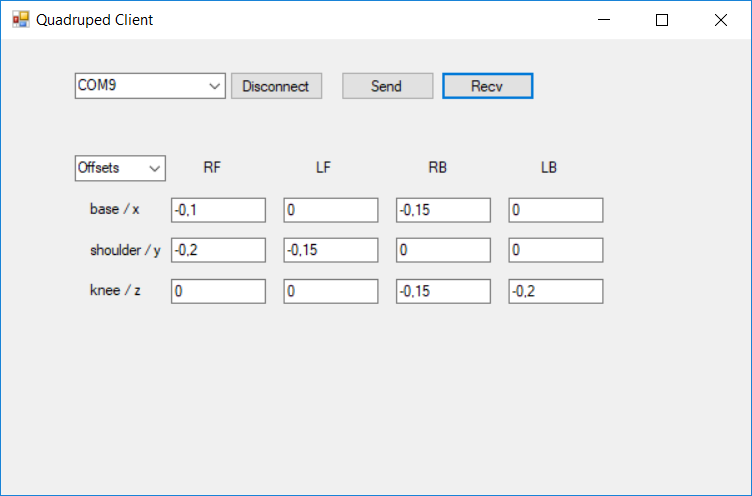
\includegraphics[width=\textwidth]{client}
	\end{minipage}
\end{figure}
A robothoz készült egy kliens program $C\sharp$-ban. Ezen ki lehet választani, melyik porton nyisson kommunikációt. Középen táblázatos formában be lehet írni minden lábhoz három értéket. \textit{Joints} és \textit{Offsets} kiválasztása esetén a szervók állása illetve offsete állítható és kérdezhető le, \textit{Positions} esetén a láb pozíciója. A \textit{Send} gombbal beállítani lehet a roboton a kiválasztott értékeket, a \textit{Recv} gombbal lekérdezni.\\ Kommunikációhoz soros portot használ. Az üzenetek egy bájt parancsból és beállítás esetén 48 bájt adatból állnak. A parancs tartalmazza, hogy beállít vagy lekérdez, és hogy csuklóállásokat, offseteket vagy pozíciót. Lekérdezés esetén válaszként megkapja a parancs bájtot és a 12 floatban tárolt adatot 48 bájton.
\section{Szimulátor}
\subsection{Számítógépes program}
\begin{figure}[h]
	\begin{minipage}{0.9\textwidth}
		\caption{Szimulátor}
		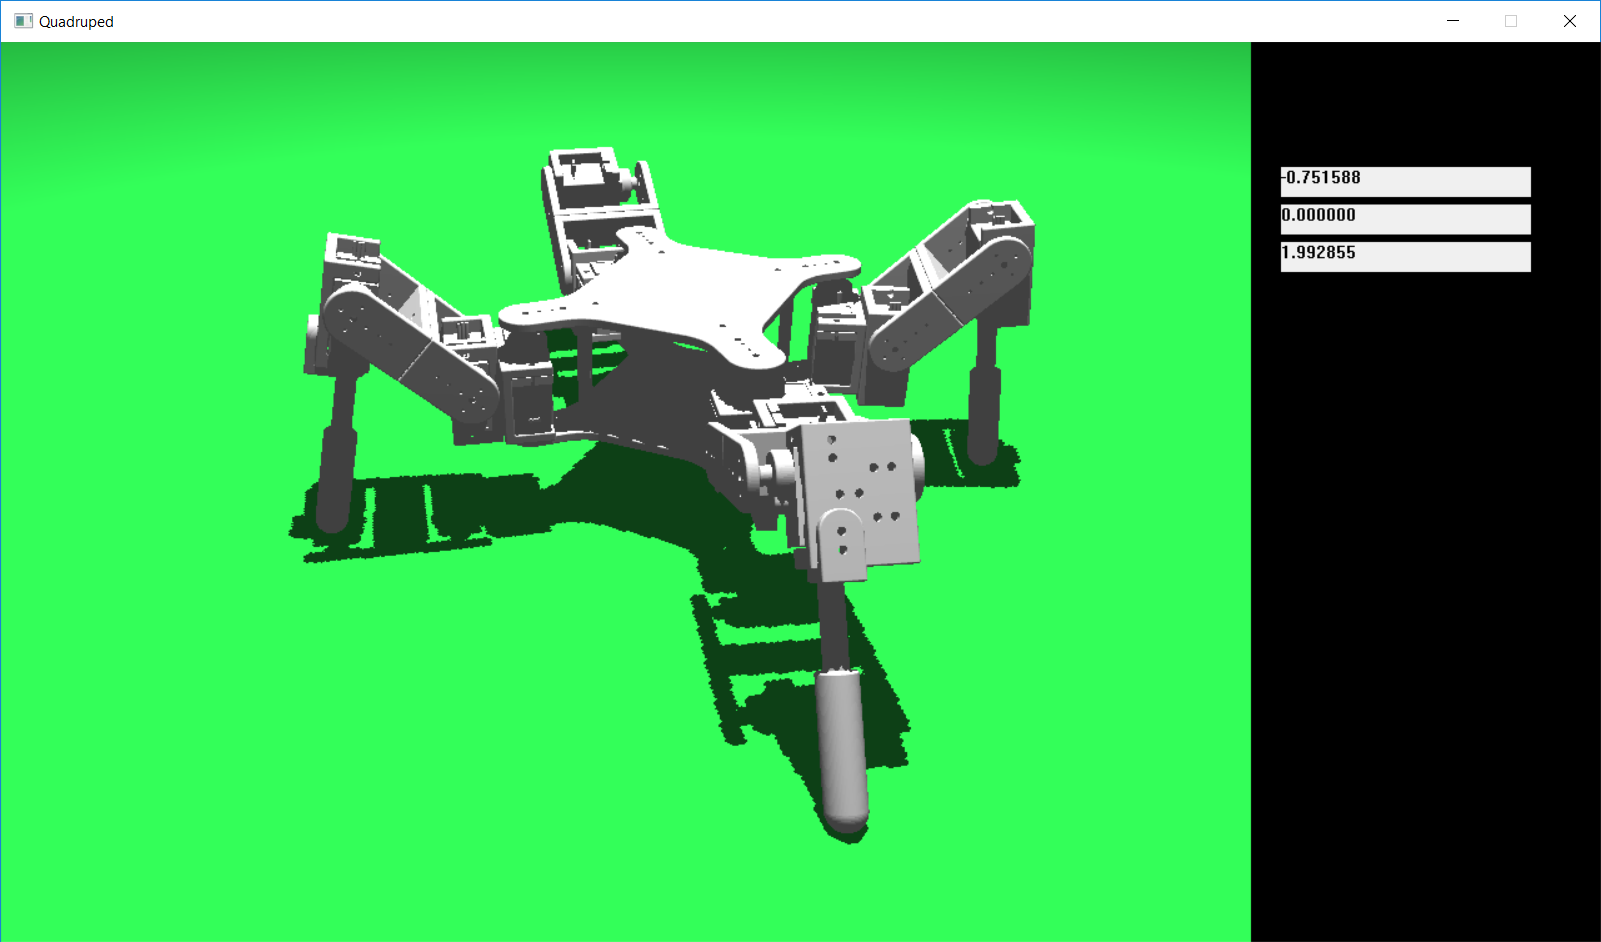
\includegraphics[width=\textwidth]{sim}
	\end{minipage}
\end{figure}
A fizikai robot előtt a mozgás teszteléséhez készült egy szimulátor C++-ban. A 3D grafikához DirectX 11-et használ, más UI elemhez windows API-t. A szép kinézet érdekében a robot modelljének elemei lettek importálva. A szerelési pontatlanságoktól eltekintve a lábak paraméterei megegyeznek a valóssal.\\
A szimulátorban nincs fizika, a robot mozgását a modell transzformálásával éri el. A szimulátor az alábbi hibákat engedi meg:
\begin{itemize}
	\item Csúszás
	\item Padlóba súllyedés, lebegés
	\item Lehetetlen egyensúlyozás
	\item Végtelen gyors mozgás
	\item Önmagába hajlás
\end{itemize}
A robot megfelelő transzformációknak köszönhetően látszik mozogni. Amikor mindegyik láb mozog, az egész robot modellje megkapja ugyanazt a transzformációt ellentétes előjellel.\\
\subsection{Áttérés fizikai robotra}
A szimulátorban megírt kód a roboton futó kódhoz hasonlóan C++-ban íródott, így túlnyomó része átírás nélkül használható volt a mikroprocesszoron. Azonban megjelentek hibák, amikre a szimulátor nem készült fel. Összeszerelés után a csuklóknak offseteik voltak. Ezt kiküszöbölni a szervók kaptak egy \textit{assemblyOffset} tagváltozót. Emellett néhány szervó ellenkező irányba forgott, mint a szimulátorban, ezért a lábak kaptak \textit{dir1, dir2, dir3} tagváltozókat, amik értéke 1 vagy -1 lehet.\\
A robot ezután már tudott járni. Az egyenes mozgást szépen végezte, viszont forgáskor nagy terpeszekbe lépett és nem volt jól kiegyensúlyozva. A lábak szétcsúsztak és földre ért a robot hasa. A \textit{WalkScript} tagváltozói állításával javult a helyzet, de a tökéletes eredmény eléréséhez az algoritmuson szükséges fejleszteni.

\end{document}
